\chapter{NLOS IS-VLP 理论基础}

\section{NLOS IS-VLP 系统概览}
首先,考虑一个典型的室内环境,如房间、办公室或超市等等,它们安装多个LED用于照明,本文在这里用一个简化的立方体模型代表房间,如图\ref{fig:typical model}所示,其中三个LED被部署在天花板上,一个装有图像传感器的设备位于空间的任意位置,与传统的VLP系统不同的是,本文提出的系统模型是通过地面的反射光来进行通信的。为了更加清晰的表示空间中的位置信息,本文考虑在房间内建立一个世界坐标系(World Coordinate System, WCS)。与大多数的VLP演示系统一样,本文选择地板平面作为X-Y平面,垂直于X-Y平面向上是Z轴的正方向。坐标系的原点O一般选择在X-Y平面的顶点。需要说明的是,这只是一种典型的模型,实际的WCS可以根据现场环境来设定。在确定了WCS之后,测量出三个LED的WCS坐标,它们将是NLOS IS-VLP系统的信标。
\begin{figure*}[!htbp]
  \centering
  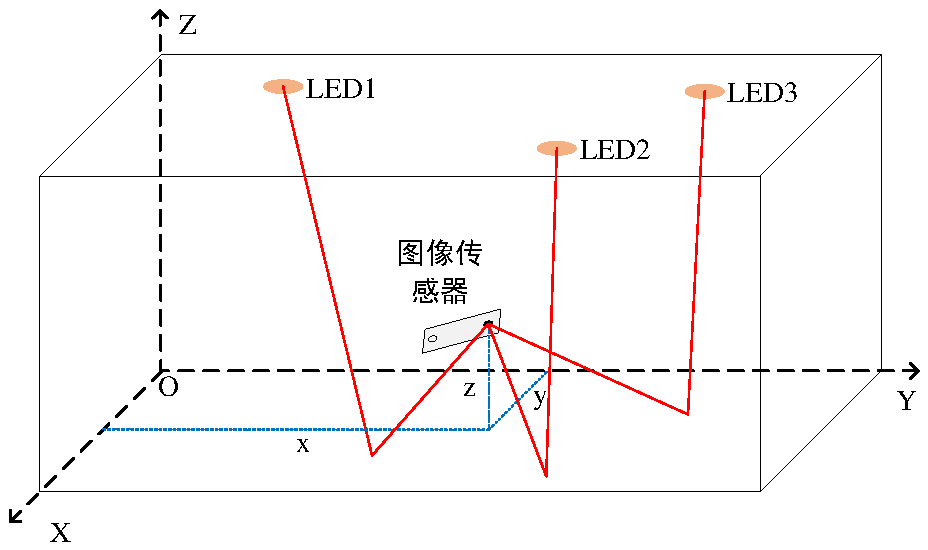
\includegraphics[width=0.7\linewidth]{FIG/system model.pdf}
  \caption{典型的非视距可见光成像定位系统几何模型}
  \label{fig:typical model}
\end{figure*}

NLOS IS-VLP系统的结构,如图\ref{fig:system-architecture}所示。在发射端,先对所有LED坐标进行编码,之后使用一个微控制器对编码进行调制,通过输出的电信号控制一个光学驱动器,最终驱动LED阵列发出可见光信号。在接收端,图像传感器在成像过程中捕捉LED阵列来自地面的反射光,通过图像处理一方面可以获得多个LED的世界坐标,另外一方面可以获取LED在地面上形成的高光点的像素坐标。然后根据高光点和LED之间的几何关系、LED的世界坐标、高光点的像素坐标以及辅助传感器的姿态信息,可以估计图像传感器的位置。

\begin{figure*}[!htbp]
  \centering
  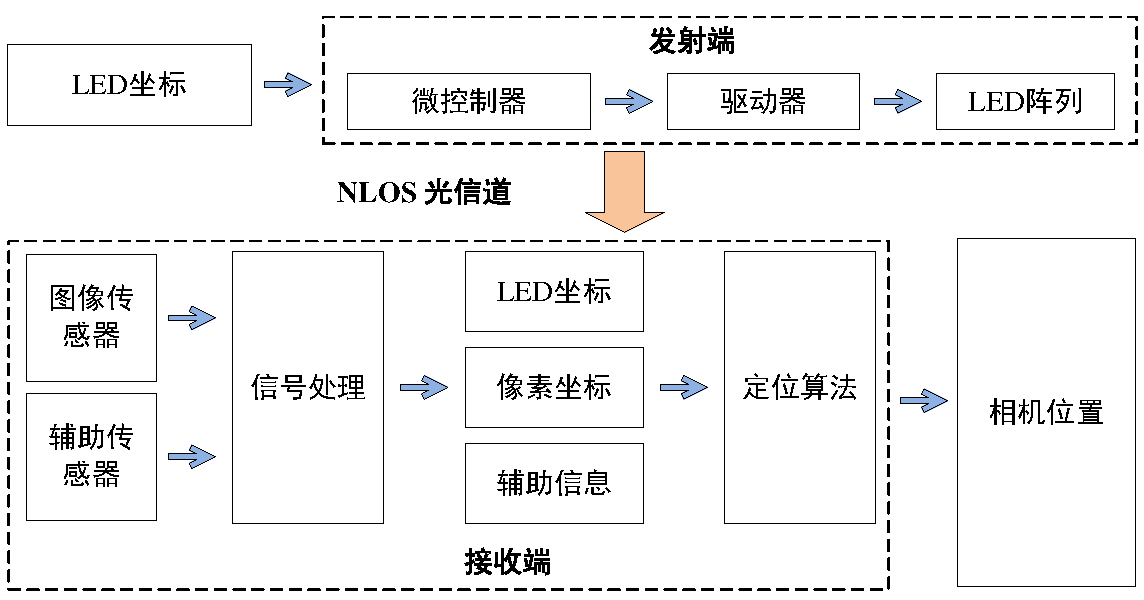
\includegraphics[width=0.85\linewidth]{FIG/2-1-2-architecture.pdf}
  \caption{非视距可见光定位的系统架构}
  \label{fig:system-architecture}
\end{figure*}

一个定位系统的一般流程分为三个步骤,分别是发射端位置信息的发送、接收端对位置信息的获取以及使用定位算法估计接收端的位置。根据图\ref{fig:system-architecture},可以知道NLOS IS-VLP系统的工作流程也是如此。

第一步:位置信息的发送。首先,要精确标定每个LED灯在设定的世界坐标系中的坐标。然后,将每个LED坐标转换成二进制数据,为了便于解调,通常会对二进制数据使用曼彻斯特编码来进行预处理。再对位置信息进行编码之后,要考虑如何将这些二进制编码转化为模拟信号,通常使用开关键控(On-off-keying, OOK)来对二进制编码进行调制,对于的“1”输出高电平,“0”输出低电平。当我们把在电脑端离线处理的编码调制的代码输入到微控制器之后,运行起来的微控制器将通过输出的高低电平来控制驱动器。驱动器其实类似于一个开关,它的一对输出节点和直流电源以及LED串联在一起,当微控制器输出高电压,驱动器出口导通,从而驱动LED发光;当微控制器输出低电平时,驱动器的出口断开,LED不发光。由此,及实现了二进制编码与LED的亮灭状态直接相关,也就是通过位置信息编码实现了对光强度的控制。这是最简单的一种调制方式,还有一些更复杂的调制方式,如脉冲宽度调制(Pulse Width Modulation, PWM)、脉冲位置调制(Pulse Position Modulation, PPM)、脉冲幅度调制(Pulse Amplitude Modulation, PAM)等等。它们将二进制编码与LED发光信号的脉冲宽度、位置以及强度等进行关联,在接收端根据这些状态信息进行解调。上述的方法是针对一个LED时的情况,在多个LED同时发送位置信息时,还需要考虑如何区分在接收端收到的混叠在一起的信息。这就依赖于复用协议,常见的复用协议有空分复用(Space Division Multiplexing, SDM)、时分复用(Time Division Multiplexing, TDM)、频分复用(Frequency Division Multiplexing, FDM)等等。在加入复用协议之后,微控制器会按照复用协议对多个LED进行调制进而控制多个LED按照复用协议产生光信号。


第二步:位置信息的接收。与LOS的情况不同,NLOS IS-VLP系统使用一个相机在低曝光模式下捕捉经过地面反射的LED光信号。对于目前大部分的演示系统来说,都是通过离线方式将每一帧低曝光度的照片输入到计算机进行处理。由于卷帘快门(Rolling Shutter, RS)效应,这些照片的内容都是一些明暗的条纹。通过图像处理技术可以获得图像的灰度值,这些灰度值的分布跟复用协议以及调制方式直接相关。一般都是先根据复用协议,分理处每一个LED对应的信号,在根据每一个LED使用的调制方案,就可以解调出每一个LED对应的编码,在经过解码就可以得到每个LED的坐标。

第三步:位置估计。首先,需要调整相机在长曝光模式下捕捉LED在反射面形成的虚像,本文称之为虚拟的LED,在照片上显示的效果为一个椭圆形状的高光区域。通过图像处理技术,可以获取该光区域高光点的像素坐标。根据投影几何原则,很容易知道虚拟LED与实际的LED关于反射面对称,由此可以获得虚拟LED在WCS下的坐标。在此之后,如果将虚拟LED的像素坐标和世界坐标输入到定位算法中,就可以估计接收端相机的位置。定位算法通常选择CV的方法,实际上也可以选择AOA算法。定位算法一般包括粗略的位置估计和后续的位置优化。

通过上述三个步骤,可以实现在NLOS的条件下实现对接收端相机位置的估计。实际上,上述三个步骤可以通过两个模块来实现,分别是NLOS OCC系统和位置估计系统。本文将在接下来的内容分别详述NLOS OCC技术理论基础和NLOS IS-VLP定位算法的基本原理。

%%%%%%%%%%%%%%%%%%%%%%%%%%%%%%%%%%%%%%%%%%%%%%
%\subsection{NLOS IS-VLP 应用场景}
%本文按照实际的需求来开展当前的工作的。一些应用场景下基于位置服务的需求,在设计VLP系统之前就已知被考虑。在过去几年中,基于WiFi、蓝牙和音频的IPS已在商业上部署,室内VLP系统更多的还是在实验室研究阶段,少有的一些商业应用也是属于试点型的工程。在本文的预期中,下面一些场景可能对可见光定位系统的需求比较大。

%\begin{enumerate}[topsep = 0 pt, itemsep= 0 pt, parsep=0pt, partopsep=0pt, leftmargin=20pt, itemindent=0pt, labelsep=6pt, label={(\arabic*)}] 
%
 %   \item 医疗场所:由于VLC技术可以兼具照明、通信与定位多功能于一体,并且没有电磁干扰,对医院等场所来说非常需要。
  %  \item 地下矿井:VLP没有电磁干扰,对矿井等场所来说非常的关键,通过VLP系统可以给实时的跟踪定位地下工作人员的位置。
   % \item 物流工厂:VLP系统在特定的环境下可以实现低成本、高精度定位。物流工厂对定位的要求比较高,同时很少了其他光源的干扰,非常适合通过密集不知LED来实现包裹的定位和跟踪。
   % \item 智慧商超:商场超市物品繁多,只有通过低成本的定位方案才能实现对每一件商品进行跟踪,这对于未来的无人化超市非常关键。
   % \item 地铁车站:地铁车站等场所经常人流量大,蜂窝网络任意产生拥挤,导致通信定位系统的失效,VLP凭借无限带宽的优势,可以避免由于多用户同时访问产生的拥塞问题,给旅客提供精准的位置服务。   
%\end{enumerate}

%总的来说,由于VLP系统无电磁干扰、无线带宽以及成本低精度高等优点,有很大的商用潜力,特别是在一些特定场所。当然,商业推广困难的主要原因还是因为前面所述的面临一些挑战,本文的主要内容就是基于如何克服这些难点,从而实现对VLP系统的快速推广。
%%%%%%%%%%%%%%%%%%%%%%%%%%%%%%%%%%%%%%%%%%%%%%%%%

\section{NLOS OCC 技术理论基础}
作为一种使用图像传感器为接收端的VLC技术,光学相机通信OCC被纳入了修订后的IEEE 802.15.7r1标准。NLOS OCC使用图像传感器通过连续曝光来捕捉反射的LED光信号,然后通过图像处理技术恢复采样信号。NLOS OCC系统模型如图\ref{fig:OCC model}所示。一个图像传感器可以看成是多个micro-PD组成的阵列,每个像素可以像PD一样独立的将光强度信号转换成像素的灰度值。根据曝光策略的不同,图像传感器可以分为全局快门和卷帘快门RS。使用电荷耦合器件(Charge Coupled Device, CCD) 的相机采用第一种曝光策略,曝光的时候所有像素同时将光信号转换成灰度值。互补金属氧化物半导体(Complementary Metal Oxide Semiconductor, CMOS)相机使用RS策略,按照逐行曝光的规则,每一行像素同时曝光。由于全局曝光的CCD相机每一帧只能对光信号进行一次采样,一次采样频率比较低,很少有OCC系统采用CCD作为接收端。而采用RS的CMOS相机采样率除了跟帧率有关之外,还跟图像传感器的行数正相关。考虑到大多数OCC系统使用CMOS相机作为接收器,本文在后续内容中只考虑这种类型。本节余下内容首先介绍RS基本原理,然后,将列出OCC系统中一些常用的调制方案以及复用协议。在此之后,将介绍OCC系统在LOS和NLOS的情况下的信道模型。
\begin{figure*}[!htbp]
  \centering
  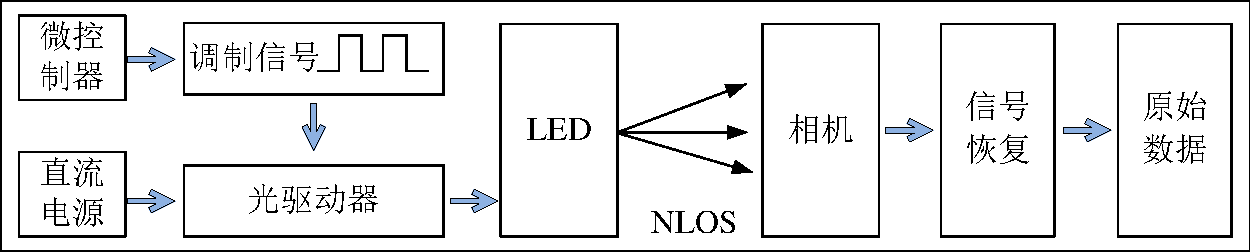
\includegraphics[width=\linewidth]{FIG/OCC modell.pdf}
  \caption{NLOS OCC系统模型}
  \label{fig:OCC model}
\end{figure*}



\subsection{CMOS相机的卷帘效应}

\begin{figure*}[!t]
  \centering
  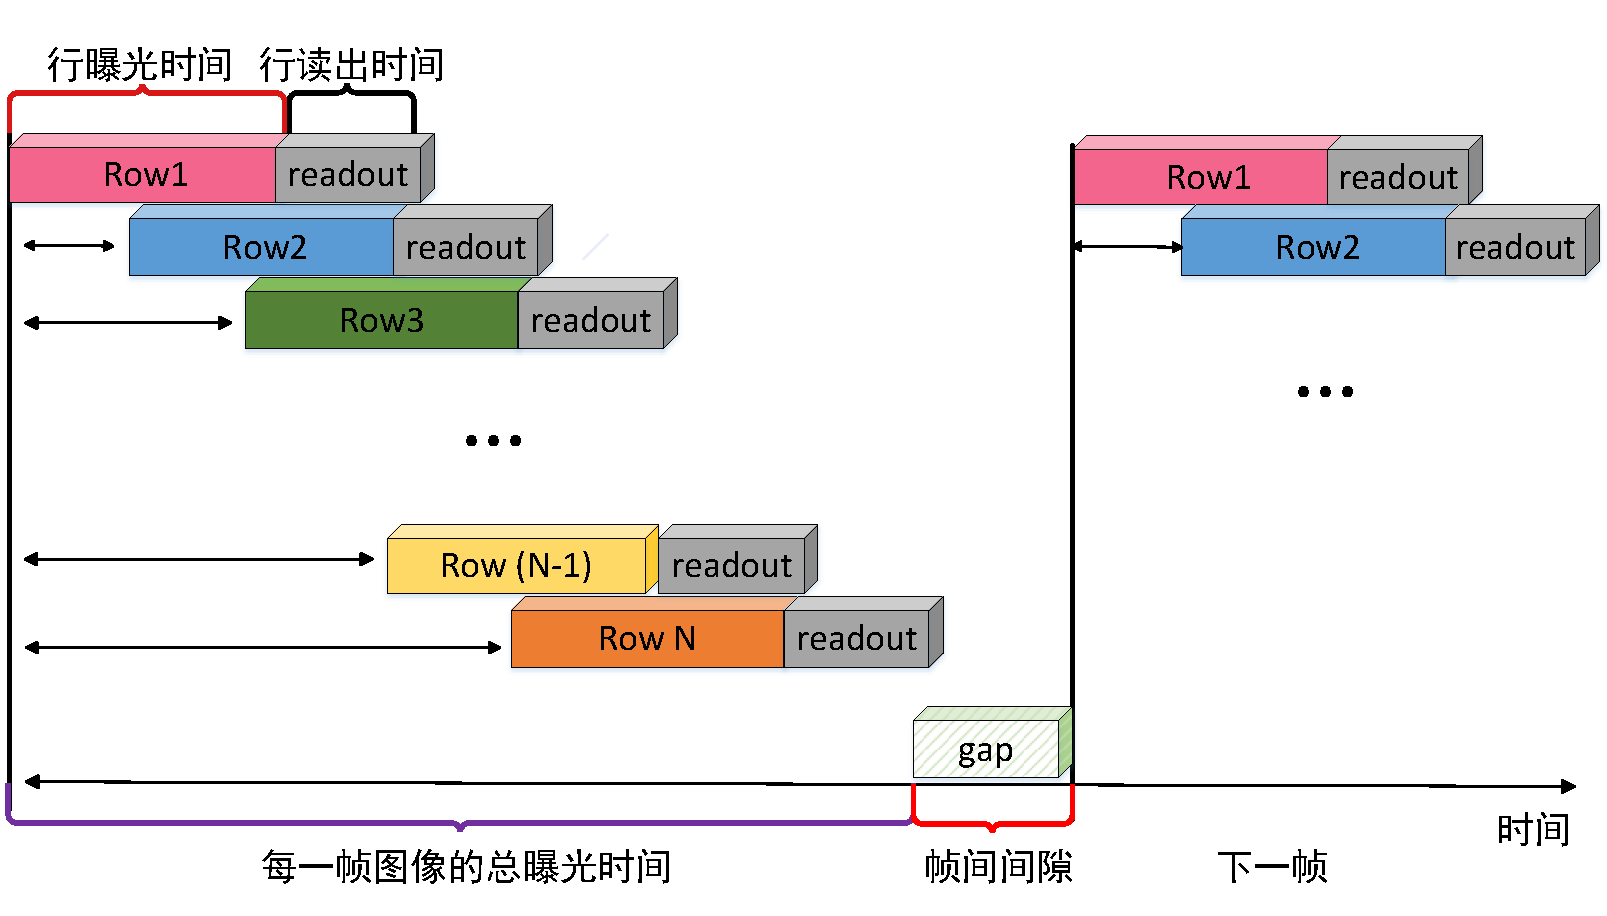
\includegraphics[width=\linewidth]{FIG/RS.pdf}
  \caption{卷帘相机曝光示意图}
  \label{fig:RS}
\end{figure*}
相机的内部快门机制决定了图像传感器中像素的曝光方式。CMOS相机RS曝光机制如图\ref{fig:RS}所示。由于其独特的电气设计,CMOS相机具有更低的功耗、更短的读出时间、更低的成本和更多的可编程性。此外,通过其逐行曝光的形式,CMOS相机理论上的最高采样频率可以达到行数与帧率的乘积。发射端LED收到驱动电路的控制,以特定的调制方式发出强度变化的光信号,处在每一行曝光时间窗对应的光信号强度跟对应行的像素值正相关。每行像素接收到的光强度会随着调制信号的变化而变化,这就导致在每个曝光期的采样信号强度不同,灰度值也会不同。最后,在拍摄的图像中会出现许多明暗相间的条纹。这就是我们所说的RS效应。OCC系统必须对接收到的每一帧图像进行图像处理,在经过复用协议的处理之后,将灰度值转换成关于行的一维离散信号,实际上就是对光强度信号的采样信号,最后再进行信号解调和解码,回复成原来的信息。

虽然LOS OCC接收到的光信号信噪比更高更易于解调,但是图像上光线直射的区域与其他区域强度区分太大导致仅有直射区域有少量的明暗条纹,这样限制了OCC系统的速率。NLOS OCC就不存在这样的问题。但是,NLOS OCC信噪比较低,系统应该设计一个合适的发射端频率并调整摄像机参数,包括快门时间、感光度ISO等,使得每幅图像上的明暗条纹的数量应尽可能多的同时对比度应尽可能高,从而最大限度地提高通信速率和降低误码率。为了实现这一目标,NLOS OCC根据奈奎斯特采样定律,采样频率应大于或等于信号最大频率的两倍,这限制了发射端的最大频率,描述如下。
\begin{equation}\label{eq:Nyquist}
    f_{t} \le f_{r}*N_{r}/2,
  \end{equation}
其中$f_r$是帧率,$N_r$是每幅图像中的像素行数,$f_t$是发射端频率。

事实上,快门时间要尽可能低,因为当快门时间过长,每行像素的曝光时间将会大于发射端信号的周期,在这种情况下,每行像素的累积采样值在曝光期内趋于饱和。也就意味着,明暗条纹只会出现在短曝光期的图像中。但是,曝光周期也不能太短,否则会造成每行像素欠曝光,图片的总亮度过暗,导致信噪比过低,解调难度变大。除此之外,由于图像传感器的感光度ISO决定了照亮一个像素需要多少个光子。因此,当ISO过高时,照亮一个像素需要的光子数过少,就会导致高光溢出,从而图像出现过曝,使明暗条纹无法区分。因此,有合理调节相机的参数,这样不仅能拍摄到清晰的明暗条纹,还能使条纹数量最大提高通信速率。


\subsection{调制与复用技术}
调制与复用技术对通信系统的性能至关重要。调制技术是一种在数字信号转换成模型信号的过程中的一种映射关系,根据这种映射关系,在接收端又可以将接收到的模拟信号转换成数字信号。这里给出了OCC系统中几种常见的调制技术,如开关键OOK、脉冲幅度调制PAM、脉冲宽度调制PWM、脉冲位置调制PPM和相移键控(Phase Shift Keying, PSK),它们的基本原理如图\ref{fig:modulations}所示。
\begin{figure}[!t]
\centering
  \begin{minipage}{0.45\linewidth}
    \centerline{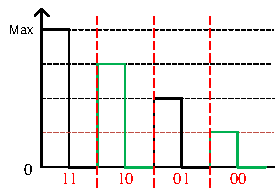
\includegraphics[width=\textwidth]{FIG/4PAM.pdf}}
    \centerline{(a) 4PAM}
  \end{minipage}
  \begin{minipage}{0.45\linewidth}
    \centerline{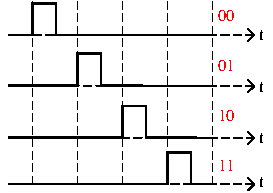
\includegraphics[width=\textwidth]{FIG/4PPM.pdf}}
    \centerline{(b) 4PPM}
  \end{minipage}\\
\vspace{10pt}
   \begin{minipage}{0.45\linewidth}
    \centerline{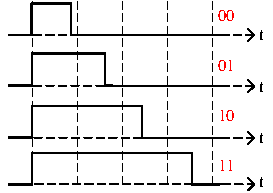
\includegraphics[width=\textwidth]{FIG/4PWM.pdf}}
    \centerline{(c) 4PWM}
  \end{minipage}
  \begin{minipage}{0.45\linewidth}
    \centerline{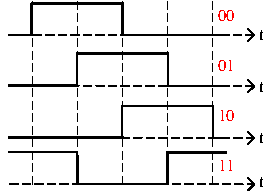
\includegraphics[width=\textwidth]{FIG/4PSK.pdf}}
    \centerline{(d) 4PSK}
  \end{minipage}
  \vfill
  \caption{几种典型的调制技术}
  \label{fig:modulations}
\end{figure}


作为一个二进制PAM,是一种最简单的调制技术,通过打开和关闭LED来传输数据位1和0。由于很容易实现并解调简单,广泛用于OCC系统中。尽管这种调制方法无法通过多级调光实现高速率传输,但它非常适用于数据传输量小的VLP系统。可以通过增加振幅的调节级别来提高符号率,如4PAM,图\ref{fig:modulations}(a)给出了4PAM的基本原理。

PPM是一种基于脉冲位置的调制方法, 如图\ref{fig:modulations}(b)所示。在一个周期内,脉冲信号的位置与传输的符号进行匹配。PPM调制技术,将一个周期划分成多个长度相同的小时间窗,脉冲持续的时间就是一个小时间窗。一周周期内,只允许一个小时间窗有脉冲信号,由此即可唯一确定的对应一个符号。要想时间较高的符号率,在相同大小的周期内需要划分更多的小时间窗来对用更多的符号数量。但是,由于相机采样的精度较低,由此时间窗不能太小,这就导致了PPM的频谱效率较低,数据速率较低。

PWM通过符号周期内的脉冲持续时间来区分不同的符号, 如图\ref{fig:modulations}(c)所示,在4PWM中,经常通过设置脉冲的占空比为0.2、0.4、0.6、0.9来方便区分不同宽度的脉冲信号。对于OCC系统,在PWM中明暗条纹的宽度比例并不一定与脉冲的占空比完全相同。这是由于多方面的原因造成的,主要是受LED的非线性和电容的滞后效应的影响,像素值通常随着脉冲持续时间的增加而增加,这使得解调变得困难。


PSK根据载波相位来表示符号, 如图\ref{fig:modulations}(d)所示。基于方波的4PSK方案在OCC系统中很常见,通过对一个符号周期内的信号相位进行判断时,很容易知道它与初始相位的差异,由此可以解调出对应的符号。4PSK调制简单,但是符号率比较低。


\begin{figure}[!t]
\centering
  \begin{minipage}{0.6\linewidth}
    \centerline{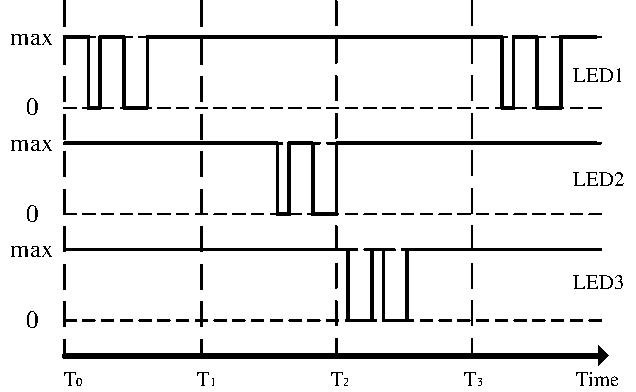
\includegraphics[width=\textwidth]{FIG/TDM.pdf}}
    \centerline{(a) TDM}
  \end{minipage}\\
\vspace{10pt}
  \begin{minipage}{0.6\linewidth}
    \centerline{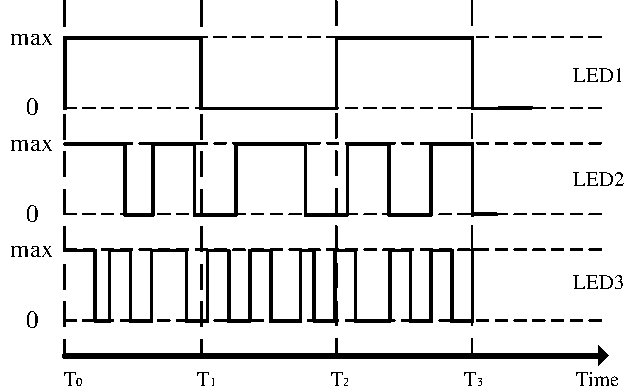
\includegraphics[width=\textwidth]{FIG/FDM.pdf}}
    \centerline{(b) FDM}
  \end{minipage}
  \vfill
  \caption{两种典型的复用协议}
  \label{fig:mutiple}
\end{figure}
在VLP系统中,接收端经常会同时接收到多个LED光信号,为了能够将多个LED一起发过来的混叠信号进行分离解调。VLP系统需要在发射端考虑复用协议,它将实现高信道利用率并减少信号间的干扰。


由于发射端LED的布局在空间上的差异,OCC系统经常使用空分复用SDM协议,多个LED同时发射光信号,相机在不同的位置捕捉到的不同LED的信号。实际上,在相机的视场角内同时捕捉到多个LED,也是可以根据SDM进行信号分离,这是由于相机每一行像素在空间上也有差异,同一行不同位置的像素虽然同时曝光,但是曝光强度跟接收到的信号强度有关,不同位置接收到的信号强度是不同的。这在很多直接视距OCC系统中,经常使用,一帧图像上面存在多个LED条纹光斑。但是在非视距场景下,由于反射光信号信噪比比较低,空间上的光强度的差异并不明显,因此单纯使用SDM,很难分离信号,这个时候使用其他的复用协议很有必要,比如常用的复用协议还有时分复用TDM、频分复用FDM、波分复用(Wave Division Multiplexing, WDM)。

TDM在时域中为每个发射端LED分配一个时隙,每个LED只允许在分配的时隙内发射其坐标信息而其他所有的LED发射功率维持不变。在这种情况下,每一个时隙内只有一个调制信号,在一个固定的周期内按照顺序依次在每一个时隙里面发送一个LED的坐标信息。在接收端捕获的每一帧图片里面,包含了很多明暗条纹,按照行数从前往后可以划分为多个区域,每一个区域的明暗条纹对应一个LED的坐标信息,如图\ref{fig:mutiple}(a)所示。

FDM是一种在通信系统里面使用最多的复用技术之一,由于其很高的信道利用率。在OCC系统中,使用方波作为载波,将信号加载在方波上,为了便于分离来自不同LED的载波信号,FDM通过调整不同载波的频率来实现这一目的。允许所有LED在同一时间传输数据,接收端对采样信号根据不同的频率将它们分开。在FDM中,通常需要在相邻的子信道之间保持一个带隙,以避免不同信号之间的干扰。考虑到大多数LED的调制带宽有限以及相机的采样频率较低,因此OCC系统中可用带宽中可包含的子通道的数量是有限的。

WDM技术在激光通信中经常使用,通过波分复用器将同一根光纤中传输的不同波长的光信号进行分离。在OCC系统中,大多数都是更具波长不同对应的颜色不同来分离信号。在基于WDM的OCC系统中,基本上所有的演示系统都是使用RGB三色LED灯来传输位置信息,根据照片上像素值对应的RGB颜色通道,来确定信号是来自哪个LED。当然,也可以使用其他颜色的LED,但是OCC系统中的波分复用器所允许的颜色数量是有限的。因为不同的颜色会导致IS上的串扰。



\subsection{OCC系统的信道模型}
OCC系统的信道模型对于系统的理论性能的分析非常重要。同时,对于基于信道模型的VLP系统来说,精准的信道建模将提高定位精度。在OCC系统中,LOS链路和NLOS链路的几何模型如图\ref{fig:channel model}所示。

\begin{figure*}[!t]
  \centering
  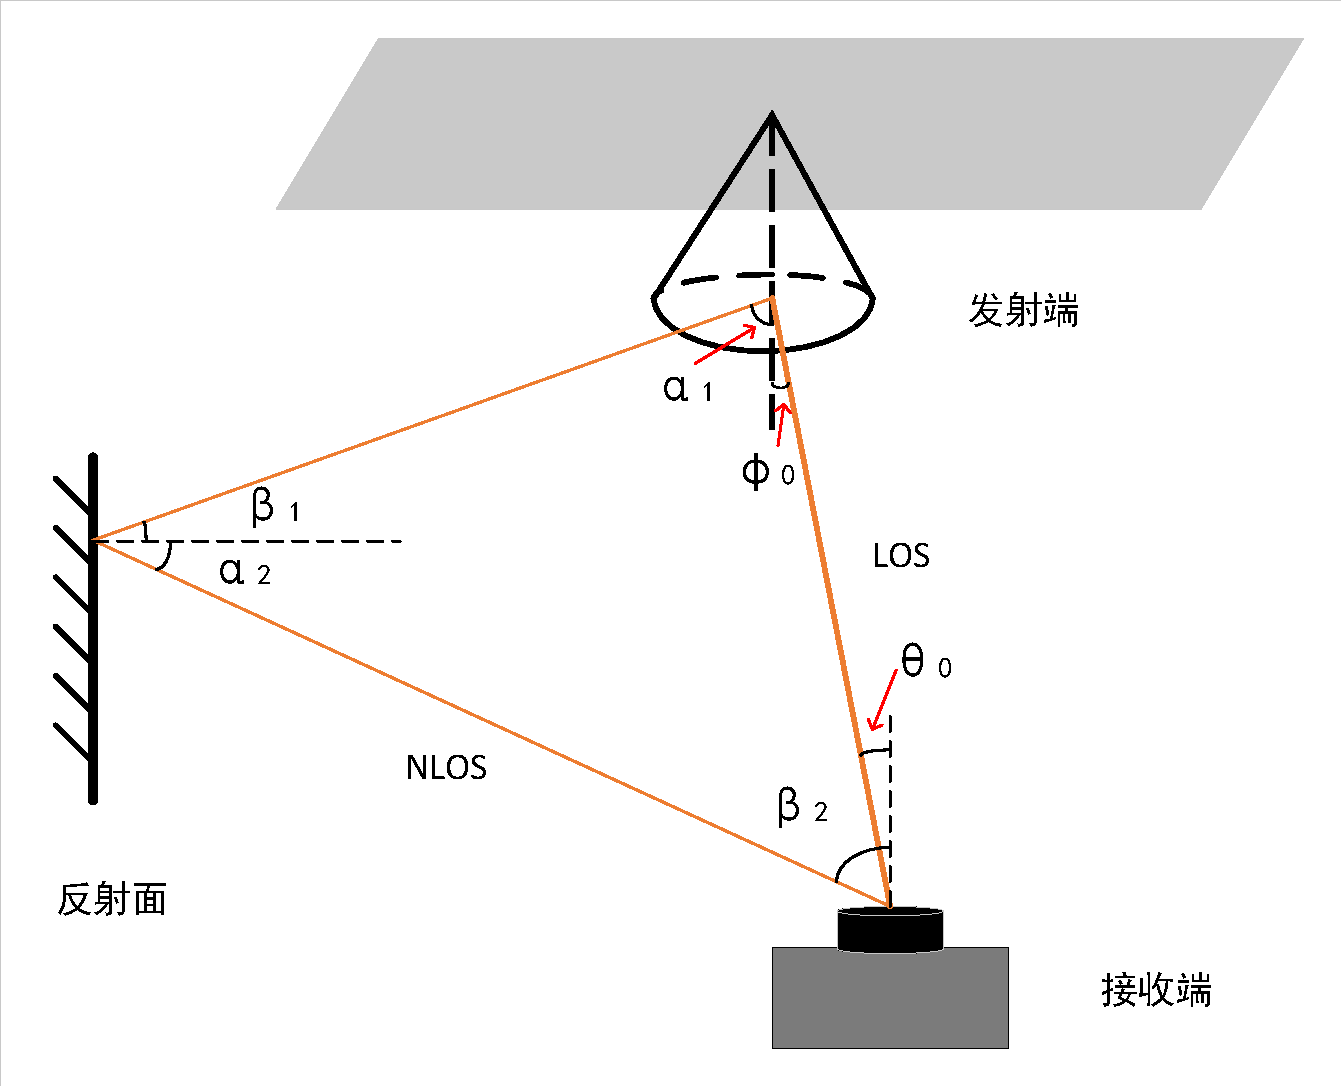
\includegraphics[width=0.85\linewidth]{FIG/channel-model.pdf}
  \caption{光学相机通信系统的直接视距链路和非直接视距链路}
  \label{fig:channel model}
\end{figure*}


目前,大多数的VLC系统信道模型都是使用朗伯模型。然而对于OCC系统来说,由于接收端类型不同,直接形式的朗伯模型并不适用于OCC系统的信道估计。主要原因在于相比于PD,图像传感器的最终采集的信息是一个像素阵列的灰度值,灰度值的大小并不能直接转化为信号功率。一个像素的灰度值与该像素区域内的光信号强度和曝光时间有关。对于OCC系统,文献\parencite{los-channel-model}给出了一个能够描述整个像素矩阵的信道增益的模型。LOS链路的信道脉冲响应可以表示为矩阵$\mathbf{H_0} = [h_0(u, v)]_{U \times V}$,其中U和V分别是图像传感器的行数和列数,$h_0(u, v)$是像素$(u, v)$的信道脉冲响应。使用单个LED和高斯混合模型,$h_0(u, v)$被估计为:
\begin{equation} \label{h0uv}
  h_{0}(u,v)=A\sum_{k=1}^{v} \frac{k^{2}c_{k}}{2\pi \sigma _{x,k}\sigma _{y,k}k_{0}^{2}}\Omega(\sigma _{x,k},\sigma _{y,k})
\end{equation}
其中,
\begin{equation} \label{omega}
  \Omega(\sigma _{x,k},\sigma _{y,k}) =\iint _{\Phi}\exp (-\frac{x^{2}}{2\sigma _{x,k}^{2}} -\frac{y^{2}}{2\sigma _{y,k}^{2}}){\mathrm{d} y}{\mathrm{d} x}
\end{equation}
并且,$A=1/a^2$,a是像素长度,$k$和$k_0$分别是相机在参考环节的放大系数。$\sigma_{x,k}$和$\sigma_{y,k}$定义为:
\begin{equation} \label{sigma xk,yk}
  \begin{cases}
    \sigma _{x,k}^{2}=(\frac{k}{k_{0}})^{2}\sigma_{i}^{'2}+ \sigma _{b,x}^{2}\\
   \sigma _{y,k}^{2}=(\frac{k}{k_{0}})^{2}\sigma_{i}^{'2}+ \sigma _{b,y}^{2}	
 \end{cases}
\end{equation}
其中$\sigma_{x,k}$和$\sigma_{y,k}$与$\sigma^′_i$表示模型的参数,$\sigma_{b,x}$和$\sigma_{b,y}$分别是图像平面上$x$和$y$方向的标准偏差。$Φ$代表以$(u, v)$为中心的邻域,其中$\sigma _{b,x}$和$\sigma _{b,y}$的定义为:
\begin{equation} \label{ax,ay}
  \begin{cases}
    \sigma _{b,x}=(u-i)(a+g)-u_{0}\\
    \sigma _{b,y}=(v-j)(a+g)-v_{0}	
 \end{cases}
\end{equation}
其中$(u_0, v_0)$和$(i, j)$分别是图像中心和离此中心最近的像素的坐标,$g$是两个像素之间的间隙。 


NLOS OCC系统不仅可以解决LOS链路受阻的问题,还可以提高通信速率。然而,大多数的NLOS OCC系统依然处于实验验证阶段,并没有给出NLOS OCC信道增益的理论模型。本文所提出的NLOS IS-VLP系统就是基于NLOS OCC技术,解决特定情况下的阻塞或阴影问题。文献\parencite{nlos-channel-model}给出了NLOS OCC信道模型,具体表达如下:
\begin{equation} \label{hlij}
h_{l}(i,j)=\iint _{\Phi}\frac{\rho A_{p}R_{t,l}(x,y)R_{r}(x,y)}{d^{2}_{t,l}(x,y)d^{2}_{c}(x,y)} \cos (\psi _{c}(x,y))dxdy
\end{equation}
其中,$A_p$和$\rho$分别表示单个像素面积和反射系数。$R_{t,l}(x, y)$和$R_{r}(x, y)$分别是LED和反射面的辐射函数。
$d_{t,l}(x, y)$是发射端$(x_{t,l}, y_{t,l}, z_t)$和反射面上点$(x, y, 0)$之间的距离,$d_{c}(x, y)$是相机与反射面之间的距离。对于一个无光泽的表面,反射遵循一阶朗伯模式。对于摄像机来说,入射角由以下公式给出:
\begin{equation} \label{phicxy}
  \psi _{c}(x,y)=\arccos(\vec{n_{l}}\cdot \vec{n_{c}})
\end{equation}
其中$\vec{n_l}$,$\vec{n_c}$分别是入射光的单位向量和图像传感器平面单位化法线。



\section{NLOS IS-VLP 算法原理}

\subsection{相机投影模型}
\begin{figure*}[!t]
  \centering
  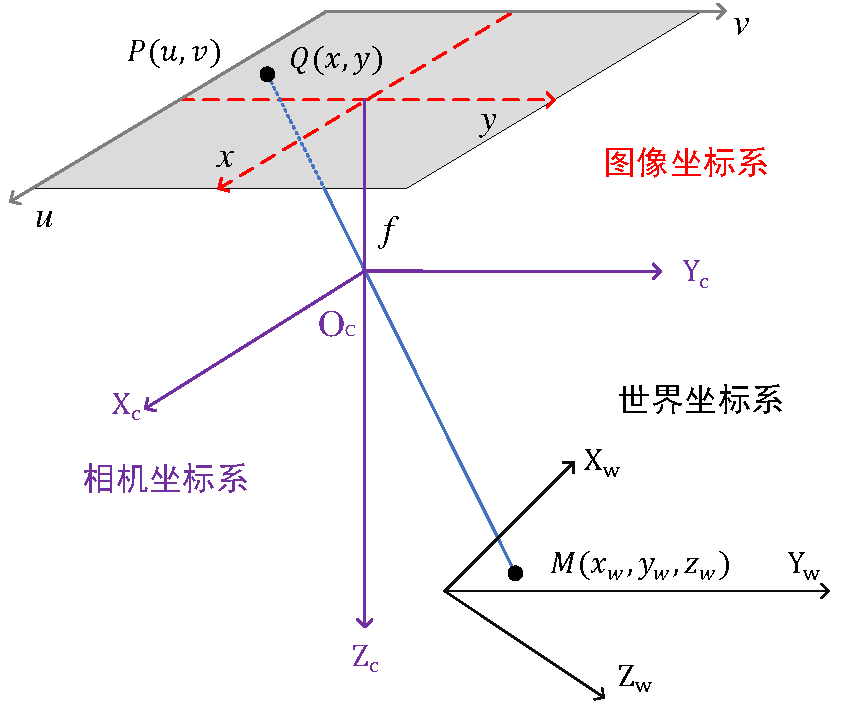
\includegraphics[width=0.6\linewidth]{FIG/CS.pdf}
  \caption{相机投影模型}
  \label{fig:CS}
\end{figure*}
成像过程可以看作是3D空间在2D平面上的投影。因此,相机视场内空间中的任何点及其投影都可以形成一组基于相似三角形的几何关系,如图\ref{fig:CS}所示。这种关系通过3D-2D投影矩阵来描述,世界坐标系WCS上坐标为$(x_w,y_w,z_w)$的点$M$投影在图像上的$P$处,像素坐标为$(u,v)$,将其转化为图像坐标上的$Q$,坐标为$(x,y)$:
\begin{equation}\label{mx:pixel-uvxy}
      \begin{bmatrix}
        u\\
        v\\
       1
       \end{bmatrix}=\begin{bmatrix}
        1/dx & 0 &u_{0} \\
         0& 1/dy &v_{0} \\
         0& 0 &1
       \end{bmatrix}\begin{bmatrix}
        x\\
        y\\
       1
       \end{bmatrix}
\end{equation}
其中,$(u_0,v_0)$是图像传感器中间点的像素坐标,$dx$和$dy$是每个像素的相邻边的物理长度。相机的焦点$O_c$被视为相机坐标系(Camera Coordinate System, CCS)的原点,点$M$在相机坐标系下的坐标为$(x_c,y_c,z_c)$,并且,点$Q$、点$O_c$与点$M$共线。根据相似三角形定律,会有:
 \begin{equation}\label{mx:cemara-xycc}
        z_{c}\begin{bmatrix}
          x\\
          y\\
         1
         \end{bmatrix}=\begin{bmatrix}
          f & 0 &0 \\
           0& f &0 \\
           0& 0 &1
         \end{bmatrix}\begin{bmatrix}
          x_{c}\\
          y_{c}\\
         z_{c}
         \end{bmatrix}
  \end{equation}
其中,$f$是相机焦距。用$\mathbf{K}$来表示原始参数矩阵:
\begin{equation}\label{eq:K}
        \mathbf{K}=\begin{bmatrix}
          f/dx & 0 &u_{0} \\
           0& f/dy &v_{0} \\
           0& 0 &1
         \end{bmatrix}
\end{equation}
 将公式(\ref{eq:K}) 和 (\ref{mx:cemara-xycc}) 代入到公式 (\ref{mx:pixel-uvxy})中, 有:
\begin{equation}\label{mx:uvxcyczc}
        z_{c}\begin{bmatrix}
          u\\
          v\\
         1
         \end{bmatrix}
         =\mathbf{K}
         \begin{bmatrix}
          x_{c}\\
          y_{c}\\
         z_{c}\\
         \end{bmatrix}
\end{equation}


最后,可以得到公式(\ref{mx:uvxcyczc}),它描述了CCS和像素坐标系(Pixel Coordinate System, PCS)之间的关系。可以使用矩阵来表达CCS和WCS之间的关系:
\begin{equation}\label{mx:world-ccww}
  \begin{bmatrix}
    x_{c}\\
    y_{c}\\
   z_{c}
   \end{bmatrix}
   =\mathbf{R}
   \begin{bmatrix}
    x_{w}\\
    y_{w}\\
   z_{w}
   \end{bmatrix}
   +\mathbf{t}
\end{equation}
其中, $\mathbf{R}$ 是旋转矩阵, $\mathbf{t}$ 是平移向量. $\mathbf{R}$是三个姿态角$\alpha$, $\beta$,和 $\gamma$的函数,可以表示为:
  \begin{equation}\label{eq:R}
    \mathbf{R}=\mathbf{R}(\alpha , \beta , \gamma)=\mathbf{R}_{x}(\alpha)\mathbf{R}_{y}(\beta)\mathbf{R}_{z}(\gamma),
  \end{equation}
其中,
  \begin{equation}\label{eq:Ra}
  \mathbf{R}_{x}(\alpha)=\begin{bmatrix}
    1 &0  &0 \\
    0 & \cos\alpha  &-\sin\alpha  \\
     0 & \sin\alpha  &\cos\alpha 
   \end{bmatrix}
  \end{equation}
   \begin{equation}\label{eq:Rb}
    \mathbf{R}_{y}(\beta)=\begin{bmatrix}
      \cos\beta &0  &\sin\beta \\
      0 & 1  &0  \\
       -\sin\beta&0  &\cos\beta 
     \end{bmatrix}
  \end{equation}
  \begin{equation}\label{eq:Rc}
    \mathbf{R}_{z}(\gamma)=\begin{bmatrix}
      \cos\gamma  &-\sin\gamma &0 \\
      \sin\gamma & \cos\gamma  &0  \\
       0&0  &1
     \end{bmatrix}
  \end{equation}
计算机视觉定位算法中经常会通过辅助传感器如惯性测量单元IMU等来测量三个姿态角,从而降低系统复杂度和提高定位精度。将公式(\ref{mx:world-ccww})代入到公式(\ref{mx:uvxcyczc})中, 有:
  \begin{equation}\label{mx:uvww}
    z_{c}\begin{bmatrix}
      u\\
      v\\
     1
     \end{bmatrix}
     =\mathbf{K}
     \begin{bmatrix}
      \mathbf{R}&\mathbf{t}
     \end{bmatrix}
     \begin{bmatrix}
      x_{w}\\
      y_{w}\\
     z_{w}\\
     1
     \end{bmatrix}
  \end{equation}
  方程组(\ref{mx:uvww}) 即为相机2D-3D投影模型。需要注意的是,这里得到的是理论的相机投影模型,然而,实际的过程会引入各种类型的误差,比如相机自身的参数误差以及成像的热噪声等等。通常,相机自身的参数误差可以通过相机标定程序来矫正。


\subsection{到达角度差 ADOA}
VLP系统经常使用基于三角测量的AOA算法。但是实际上,AOA算法比较复杂,在基于PD的VLP系统中通常是用PD阵列构建关于所有PD的AOA误差的最小二乘法来估计接收端位置。在IS-VLP系统中,通过一种改进的AOA算法来进行定位,这种方法主要是基于角度差关于不同坐标系的不变性,因此被称为到达角度差(Angel Deference of Arrival, ADOA)。如图\ref{fig:AOA}所示,显然有:
\begin{equation}\label{eq:theta=beta}
\theta=\phi
\end{equation}
其中,在PCS中,$\theta$根据针孔相机模型以及$M_1$和$M_2$在图像传感器上面的投影点$P_1$和$P_2$的像素坐标很容易得到:
\begin{equation}\label{eq:thetaAOA}
\theta=\arccos{\frac{\overrightarrow{O_cO_1}\overrightarrow{O_cO_2}}{O_cO_1\cdot O_cO_2}}
\end{equation}
同理,在WCS中有:
\begin{equation}\label{eq:betaAOA}
\phi=\arccos{\frac{\overrightarrow{O_cM_1}\overrightarrow{O_cM_2}}{O_cM_1\cdot O_cM_2}}
\end{equation}
将公式(\ref{eq:betaAOA})和(\ref{eq:thetaAOA})代入到公式(\ref{eq:theta=beta})中,可以得到一个关于相机原点在WCS下的坐标的方程组,当发射端有3个以上的LED两两构建一组这样的方程组就可以计算出相机在WCS下的位置。
\begin{figure*}[!htbp]
  \centering
  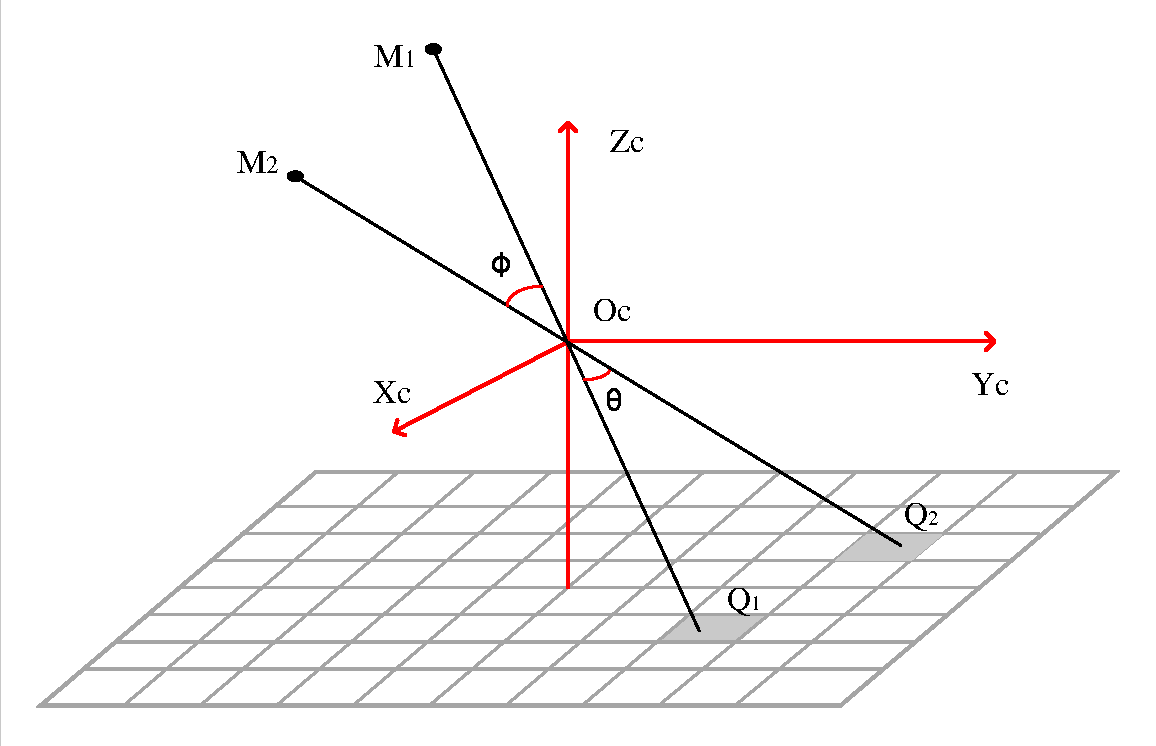
\includegraphics[width=0.8\linewidth]{FIG/AOA.pdf}
  \caption{ADOA定位算法}
  \label{fig:AOA}
\end{figure*}



\subsection{计算机视觉}
IS-VLP中计算机视觉算法主要分为两种类型。首先是直接解投影方程,即相机位置和姿态是方程的解。由于目标值是为了求解相机焦点$O_c$在世界坐标系中的坐标, 假设为$(x_R,y_R,z_R)$,而相机焦点在相机坐标系中的坐标是$(0, 0, 0)$。因此,将$(x_R,y_R,z_R)$和$(0, 0, 0)$带入到公式(\ref{mx:world-ccww}),有:
  \begin{equation}\label{eq:target}
    (x_R,y_R,z_R)^{T}=-\mathbf{R}^{-1}\mathbf{t},
  \end{equation}
等式(\ref{eq:target})意味着目标的求解可以转换成求解 $-\mathbf{R}^{-1}\mathbf{t}$。通过多对LED与其在图像传感器上的投影点对应的2D-3D投影关系,构建多个形如(\ref{mx:uvww})的非线性方程组,即可求出$\mathbf{R}$和$\mathbf{t}$,进而得出目标值。通常最少需要3组这样的非线性方程组,才能唯一确定$\mathbf{R}$和$\mathbf{t}$,从而唯一确定$(x_R,y_R,z_R)$。
 然而,由于相机参数误差以及投影点像素坐标估计误差以及测量误差等因素的存在,导致上述的非线性方程组无解,因此通常使用最小二乘法的方法将上述等式转化为优化问题。比较常见的就是重投影误差最小化算法,具体可以表示为:
  \begin{equation}\label{mx:reprojection}
    \begin{bmatrix}
      x_R\\
      y_R\\
     z_R
     \end{bmatrix}
     =\mathop{\arg\min}\limits_{}\sum_{i=1}^{N} \left \| 
     z_{ci}
     \begin{bmatrix}
      u_{i}\\
      v_{i}\\
     1
     \end{bmatrix}
     -\mathbf{K}
     \begin{bmatrix}
       \mathbf{R} &\mathbf{t}
     \end{bmatrix} 
     \begin{bmatrix}
      x_{wi}\\
      y_{wi}\\
      z_{wi}\\
     1
     \end{bmatrix}
      \right \| 
     _{2}^{2}
  \end{equation}

  第二种方法是N点透视几何(Perspective-N-Point, PNP) 算法。最经典的是P3P算法,如图\ref{fig:PNP}所示,在已知A,B,C的世界坐标以及其投影点a,b,c的情况下,根据余弦定律,在三角形$\triangle aOc$、$\triangle aOb$和$\triangle bOc$中, 首先可以计算出角$\angle aOc$、$\angle bOc$以及$\angle aOb$。进而得到$\angle AOC$、$\angle BOC$以及$\angle AOB$,这里的思路和ADOA算法基本上是一致的。不过P3P后面是更具OA、OB以及OC三者之间的比例关系,以及三者自身位置已知,进而确定O的世界坐标。需要注意的是,P3P需要3个参考点在同一平面,并且存在四个解的情况,在VLP系统中,需要通过实际情况下的集合范围约束来剔除其他解。PNP算法在计算机视觉领域使用特别多,可以直接调用OpenCV里面的SolvePNP函数进行运算。
\begin{figure*}[!t]
  \centering
  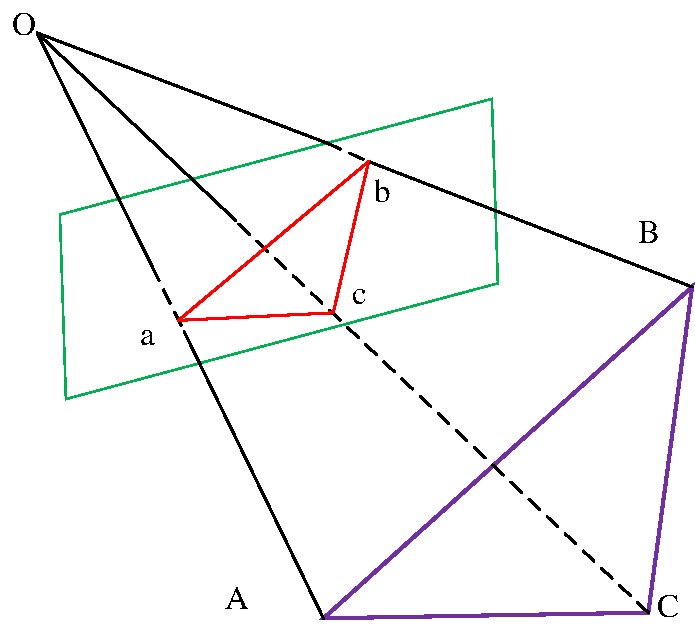
\includegraphics[width=0.4\linewidth]{FIG/PNP.pdf}
  \caption{单点透视几何}
  \label{fig:PNP}
\end{figure*}


\subsection{融合定位算法}
越来越多的研究工作开始考虑多算法协作定位和多传感器融合定位,这种融合定位的思路,一方面可以使定位系统更加灵活,另外一方面可以大大提高系统的鲁棒性。

多算法协作定位是一种利用两种或两种以上的经典定位算法来估计待估位置的方法,通常分类两种类型,第一种是通过对两种算法的定位结果进行耦合得到最终的结果,这种方法主要是为了解决单一算法在抵抗干扰时的不稳定性。第二种算法是通过两种算法分部定位的思路来降低计算复杂度。

多传感器融合定位,最常见的是惯性测量单元IMU和图像传感器组合,实现任意姿态下的3D定位,还有一些使用PD和图像传感器融合的VLP系统。这种多传感器融合,利用各种传感器提供的信息进行互助,一方面可以提高定位的精度,另外一方面可以提高定位系统的鲁棒性。特别是对于VLP系统来说,在使用辅助传感器的情况下,可以减少对视场角内同时捕捉多个LED的限制。


\subsection{基于机器学习的定位及优化算法}
随着机器学习的流行,将机器学习应用于各种领域的研究工作非常多。其中,就有一些工作研究了基于机器学习的可见光定位及优化算法。目前,使用比较多的主要有三种机器学习模型,分别是强化学习(Reinforcement Learning, RL)、人工神经网络(Artificial Neural Network, ANN)以及循环神经网络(Recurrent Neural Network, RNN)。

\begin{figure*}[!b]
  \centering
  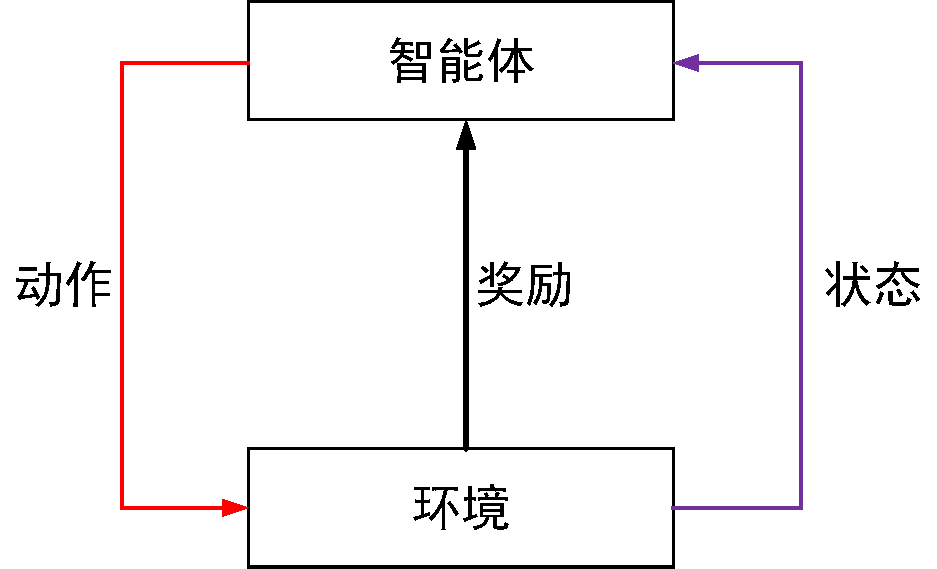
\includegraphics[width=0.5\linewidth]{FIG/RL.pdf}
  \caption{强化学习过程}
  \label{fig:RL}
\end{figure*}
强化学习RL,区别于监督学习和无监督学习,是机器学习三大类别之一。RL的基本思路是计算机通过调整自身策略来获取最大化的回报,而策略的调整就取决于跟环境互动的结果。RL的示意图如图\ref{fig:RL}所示,智能体没做出一次行为,环境都会根据该行为造成的状态变化来及时的反馈一个奖励信号给智能体,奖励信号的大小来指示行为的好坏。智能体更具奖励信号的大小和环境的当前状态来判断下一步的行为。通过这样不断的反馈和判断,最终做出适应环境的最优策略。RL的过程可以看成是一种试错行为,智能体无法知道自己的每一步行为是好是坏,但是可以根据环境的反馈来知道上一次行为是否恰当,从而选择是否继续跟随上一次的行为策略。


在NLOS IS-VLP系统中,容易受到各种测量误差的影响导致定位误差过大,LED投影点的像素估计误差、相机的姿态角的测量误差等。通过引入RL到NLOS IS-VLP系统中,由于测量信号包含误差,每一次的动作就是对测量信号进行微调,由此将改变环境状态,得到一个新的接收端的位置,将此位置反代入到定位算法中,来计算此时的重投影误差,结果来指导奖励信号的大小,模值变小是奖励,模值变大是惩罚。


\begin{figure*}[!b]
  \centering
  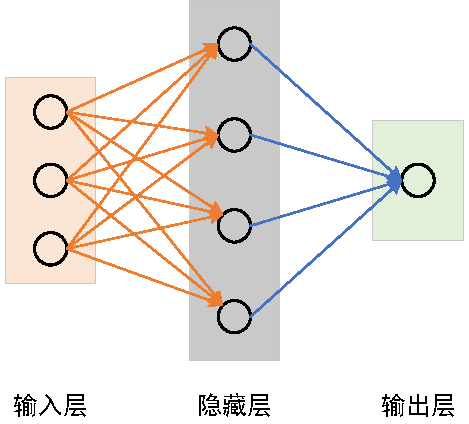
\includegraphics[width=0.5\linewidth]{FIG/ANN.pdf}
  \caption{基本的神经网络模型}
  \label{fig:ANN}
\end{figure*}
人工神经网络ANN是对人类大脑神经元网络的一种抽象和建模,通过模拟神经元的连接规则构建一种由大量节点互相连接的运算模型。图\ref{fig:ANN}展示了一个最简单的神经网络模型,模型最左边的为输入层,中间为隐藏层,最右边为输出层。需要注意的是,实际的神经网络模型输入输出以及中间隐藏神经元的个数是由实际的需求来确定的,同样,中间隐藏层的层数也是不固定的。网络中的神经元也称为节点,每两个节点之间都有一个与之对应的权重,每一个节点都有一个激活函数,他将决定对神经元的激活或抑制。激活函数的输入为上一层所有节点的加权值,激活函数是一种非线性函数,如果缺少非线性激活函数的作用,再复杂的神经网络的输出都是输入神经元的线性组合而已。在这种多层和大量神经元组合的结构中加入非线性激活函数,将大大提高网络的非线性表达能力以及容错能力。

BP神经网络作为最经典的神经网络模型之一,将误差反向传播算法应用于多层前馈神经网络中,可以对网络权重的动态调整。BP网络包含信号前传和误差反传两个步骤。在模型训练的时候,先进行信号的正向传播,输出的信号与期望值之间的误差通过反向传播流程逐层分摊,最后每一层根据自身的误差调整权重,从而完成模型的一次优化过程。

针对NLOS IS-VLP系统这种输入信号与输出位置坐标之间的非线性映射关系,可以通过训练BP神经网络模型来实现位置估计。目前已经有的研究工作中,将指纹数据、RSS和LED坐标等作为网络的输入,接收端的位置作为输出来训练网络,通过得到的模型来测试,定位精度相对于传统算法也很大的提高,并且抗干扰能力也有增强。

循环神经网络强调信号在时间上的先后关系,前一个时刻的信号会对后一刻的信号产生影响。基本的循环神经网络模型如图\ref{fig:RNN}所示,网络中的隐藏层以连续时刻的形式向后传递。RNN的这种结构非常适合处理基于时间序列的数据类型。对于定位与跟踪系统来说,由于定位结果在时间上的连续性,因此可以通过RNN来优化跟踪轨迹。对于NLOS IS-VLP系统来说,经常一帧图像对应一个相机的位姿,因此,通过RNN学习连续视频帧的关系,一方面可以优化定位结果,另外一方面在视距被阻挡的时候,可以通过RNN结合前一帧的信息来预测当前帧的定位结果。
\begin{figure*}[!htbp]
  \centering
  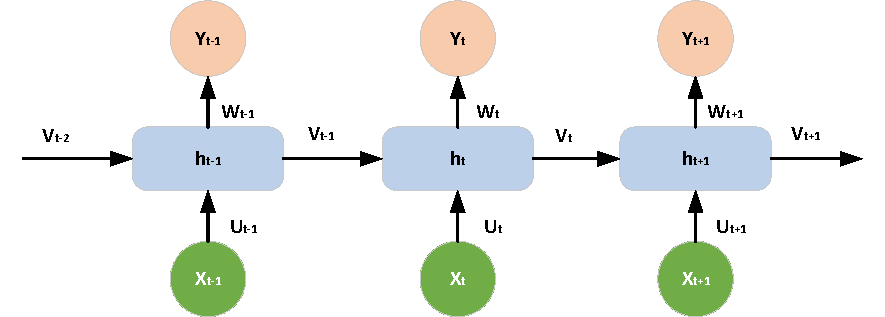
\includegraphics[width=\linewidth]{FIG/RNN.pdf}
  \caption{基本的循环神经网络模型}
  \label{fig:RNN}
\end{figure*}

\section{本章小结}
 本章主要介绍了NLOS IS-VLP系统的理论基础。首先介绍了典型的NLOS IS-VLP系统的几何模型和系统工作流程,接着根据NLOS IS-VLP系统流程可以分成两个模块NLOS OCC系统和定位系统,分别介绍了NLOS OCC的基础理论以及NLOS IS-VLP算法的基本原理。


